%!TEX root = main.tex
\section{Kontrollhandske}

\begin{figure}
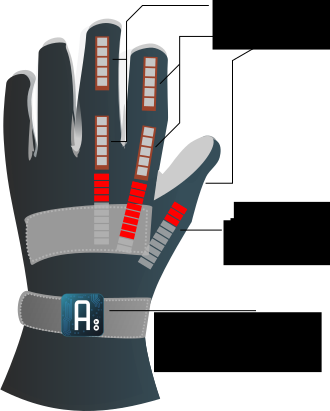
\includegraphics[height=0.9\textheight]{img/kontrollhandske}
\caption{Konceptskiss över kontrollhandsken.Flexsensorerna överför önskad vinkel till robothanden, och de röda ledlamporna återkopplar robothandens tryck till användaren. Fler röda ledlampor tända betyder högre tryck.}
\end{figure}

Robothanden styrs med hjälp av en handske som användaren bär på sin hand. Med hjälp av 6 töjningsresistorer mäts vinklar från användarens tumme, pekfinger och långfinger.
Via en liten mikrokontroller på handsken (Arduino Micro) skickas resistansförändringar från töjningssensorer vidare via Bluetooth till Robothanden. Robothanden skickar i sin tur tillbaka det uppmätta trycket som återkopplas till användaren via ledlampor på varje finger. Ju högre tryck ju fler lampor kommer att tändas.
Följande komponenter används för handsken:

\begin{itemize}
	\item Tunn handske
	\item Arduino Micro
	\item Bluetooth Mate Silver
	\item Töjningsresistorer
	\item Ledlampor
	\item Batteri
\end{itemize}

%	\item Trycksensorer
%snabbhet
%säkerhet
%prestanda






